\chapter{Pathogenic bacteria can effect the endogenous actin cytoskeleton}\label{ch:vibrio}

\section[Abstract]{Abstract\footnotemark}
\textit{Vibrio cholera} has multiple ways to interfere with a host cell’s actin cytoskeletal system. I collaborated with two projects to better understand the different pathways that gram-negative \textit{Vibrio} bacteria can commandeer the actin cytoskeleton. The actin cytoskeleton is an ideal target for pathogenic bacteria for diverse reasons depending on the pathogen. The actin cytoskeleton can be used to prevent or induce the pathogen's phagocytosis as well as facilitate their movement into, around, and out of host cells \citep{liverman_arp2/3-independent_2007}. 

The first collaboration with Tom Burke in the Kovar lab focused on the mechanism of actin nucleators VopL and VopF. These \textit{Vibrio} nucleators assemble actin into unproductive filament. There was controversy surrounding how these proteins were able to nucleate actin filaments and we presented a solution to this controversy, showing that in the presence of physiological conditions that VopL and VopF bind to the pointed ends of F-actin. With the second collaboration with the Kudryashov lab at The Ohio State University, I used single-molecule TIRF to visualize the effect of ACD toxin formed actin oligomers on Ena/VASP. The Kudryashov lab had previously found that these toxic oligomers effect formin elongation \citep{heisler_acd_2015}, and we expanded this study to other endogenous actin assembly factors. 

Overall these two works contribute to understanding the role that pathogenic bacteria can interfere with a host's actin cytoskeleton. Understanding how \textit{Vibrio} bacteria can hijack the endogenous actin system allows us to better fight the disease-causing bacteria. I have presented below the parts of the collaborations that I had a role collecting and analyzing and focus on the aspects that are relevant to my contribution. 

\footnotetext{Citations for chapter: [1] Thomas A. Burke, Alyssa J. Harker, Roberto Dominguez, and David R. Kovar. The bacterial virulence factors VopL and VopF nucleate actin from the pointed end. \textit{The Journal of Cell Biology}, March 2017. [2] Elena Kudryashova, David B. Heisler, Blake Williams, Alyssa J. Harker, Kyle Shafer, Margot E. Quinlan, David R. Kovar, Dimitrios Vavylonis, and Dmitri S. Kudryashov. Actin Cross-Linking Toxin Is a Universal Inhibitor of Tandem-Organized and Oliogmeric G-Actin Binding Proteins. \textit{Current biology}, 28{10}:1536-1547.e9, May 2018.}

\section{Introduction}\label{ch04-introduction}
Bacterial toxins can effectively compromise a host cell's functions with relatively few molecules, even leading to cell death. These toxins can target signaling cascades (ex. cGMP, adenylate cyclase) or inhibit other enzymes important for cellular processes such as protein synthesis \citep{henkel_toxins_2010}. As the actin cytoskeleton is important for many cellular processes, it is commonly targeted by bacterial toxins. The actin cross-linking domain toxin (ACD) of \textit{Vibrio} species and related bacterial genera are delivered to host cells by type 1 (MARTX toxin) \citep{sheahan_identification_2004} or type VI (VgrG1 toxin) secretion systems \citep{pukatzki_type_2007}. ACD catalyzes formation of actin oligomers through covalent crosslinking of Lys\textsuperscript{50} in subdomain 2 of an actin monomer with Glu\textsuperscript{270} in subdomain 3 of another actin monomer by an amide bond \citep{kudryashov_connecting_2008,kudryashova_glutamyl_2012}. This results in an oligomer that is not suitable for further actin polymerization because the two monomers are oriented similar to actin subunits along the short pitch of an actin filament, except that subdomain 2 has a major twist, disrupting the normal interface for further monomer binding \citep{kudryashov_connecting_2008}.  

However, though there is a high concentration of actin, only a few ACD molecules are secreted into the host cell. Using in vitro determined rates of ACD activity, it would take more than 6 months to covalently crosslink half of all the cytoplasmic actin with a single ACD molecule. This is beyond the timescale for in vivo measurements of monolayer disruption \citep{kudryashova_glutamyl_2012, heisler_acd_2015}. Previously, in a collaboration with the Kudryashov lab, we found that ACD is effective not by sequestering monomers as previously thought but by using actin oligomers to target formins. \citep{heisler_acd_2015}. We found that ACD formed toxic actin oligomers that blocked formin-mediated actin polymerization and nucleation. However, the mechanism of how these ACD-formed oligomers block formin activity remains unclear. 

Another way that bacteria target the actin cytoskeleton is through type III secretion factors VopF (\textit{Vibrio cholerae}) or VopL (\textit{Vibrio parahaemolyticus}) (VopL/F) \citep{tam_type_2007,liverman_arp2/3-independent_2007}. VopL/F contain three tandem WASP homology 2 (WH2) motifs followed by a VopL C-terminal Domain (VCD) that facilitates dimerization (Figure \ref{fig:vop}A). This places VopL/F into the class of WH2 nucleators such as cordon-bleu and Spire \citep{qualmann_new_2009}. The WH2 domain is able to bind to actin monomers in the target-binding cleft between actin subdomains 1 and 3 to facilitate actin filament nucleation \citep{namgoong_mechanism_2011}. The mechanisms of the WH2 nucleators are not as well studied as other nucleators, Arp2/3 complex and formins. 

VopL/F have a 32\% sequence identity and 72\% sequence similarity and contain the same domain organization, though two competing mechanistic models had been previously proposed. Two groups had proposed that VopL nucleates actin filaments from the pointed end and then remains associated with the new filament for only a short time \citep{namgoong_mechanism_2011, yu_mechanism_2011} and another group had proposed that VopF binds to the barbed end of growing F-actin and can also sever filaments \citep{pernier_dimeric_2013}. The crystal structure of VopL in complex with actin was solved and showed that the VCD dimer binds to three actin monomers in an arrangement that is close to F-actin and allows each actin subunit to bind to a WH2 motif \citep{zahm_bacterial_2013}. We set out to clear up this controversy by using single-molecule TIRFM to visualize VopL/F binding to filaments \citep{burke_bacterial_2017}. 

\section{Results}\label{ch04-results}

\subsection{Ena/VASP is inhibited by actin crosslinking toxins}\label{ena-acd-oligomers}
Our previous study showed that formin mediated elongation of F-actin is blocked by ACD oligomers in a concentration dependent manner \citep{heisler_acd_2015}. We measured the IC\textsubscript{50} of ACD oligomer inhibition of mDia1 to be 1.2$\pm$0.6 nM. To further understand the mechanism of how these ACD oligomers affect actin assembly factors we measured their effect on Ena/VASP. We used two-color TIRFM to directly visualize the assembly of 1.5 $\mu$M Mg-ATP-actin monomers (15\% Oregon green-labeled) with 15 pM fluorescently labeled SNAP(549)-Ena$\Delta$L (referred to as Ena) (Fig. \ref{fig:ena-bundlers}A) and human fascin or fly fascin, Singed.We used single-molecule TIRF microscopy to measure the dynamics of single Ena/VASP proteins in the presence of increasing concentration of ACD oligomer in the presence of fly profilin, chickadee. We found that Ena/VASP is affected by the ACD oligomers and will cap filaments, blocking growth. We calculated the percentage of capped filaments over a range of ACD oligomers and found that with increasing ACD oligomers, Ena/VASP capped more filaments. We also observed that the run length of Ena/VASP was much longer as a cap than as an elongation factor. 

\begin{figure}
\centering
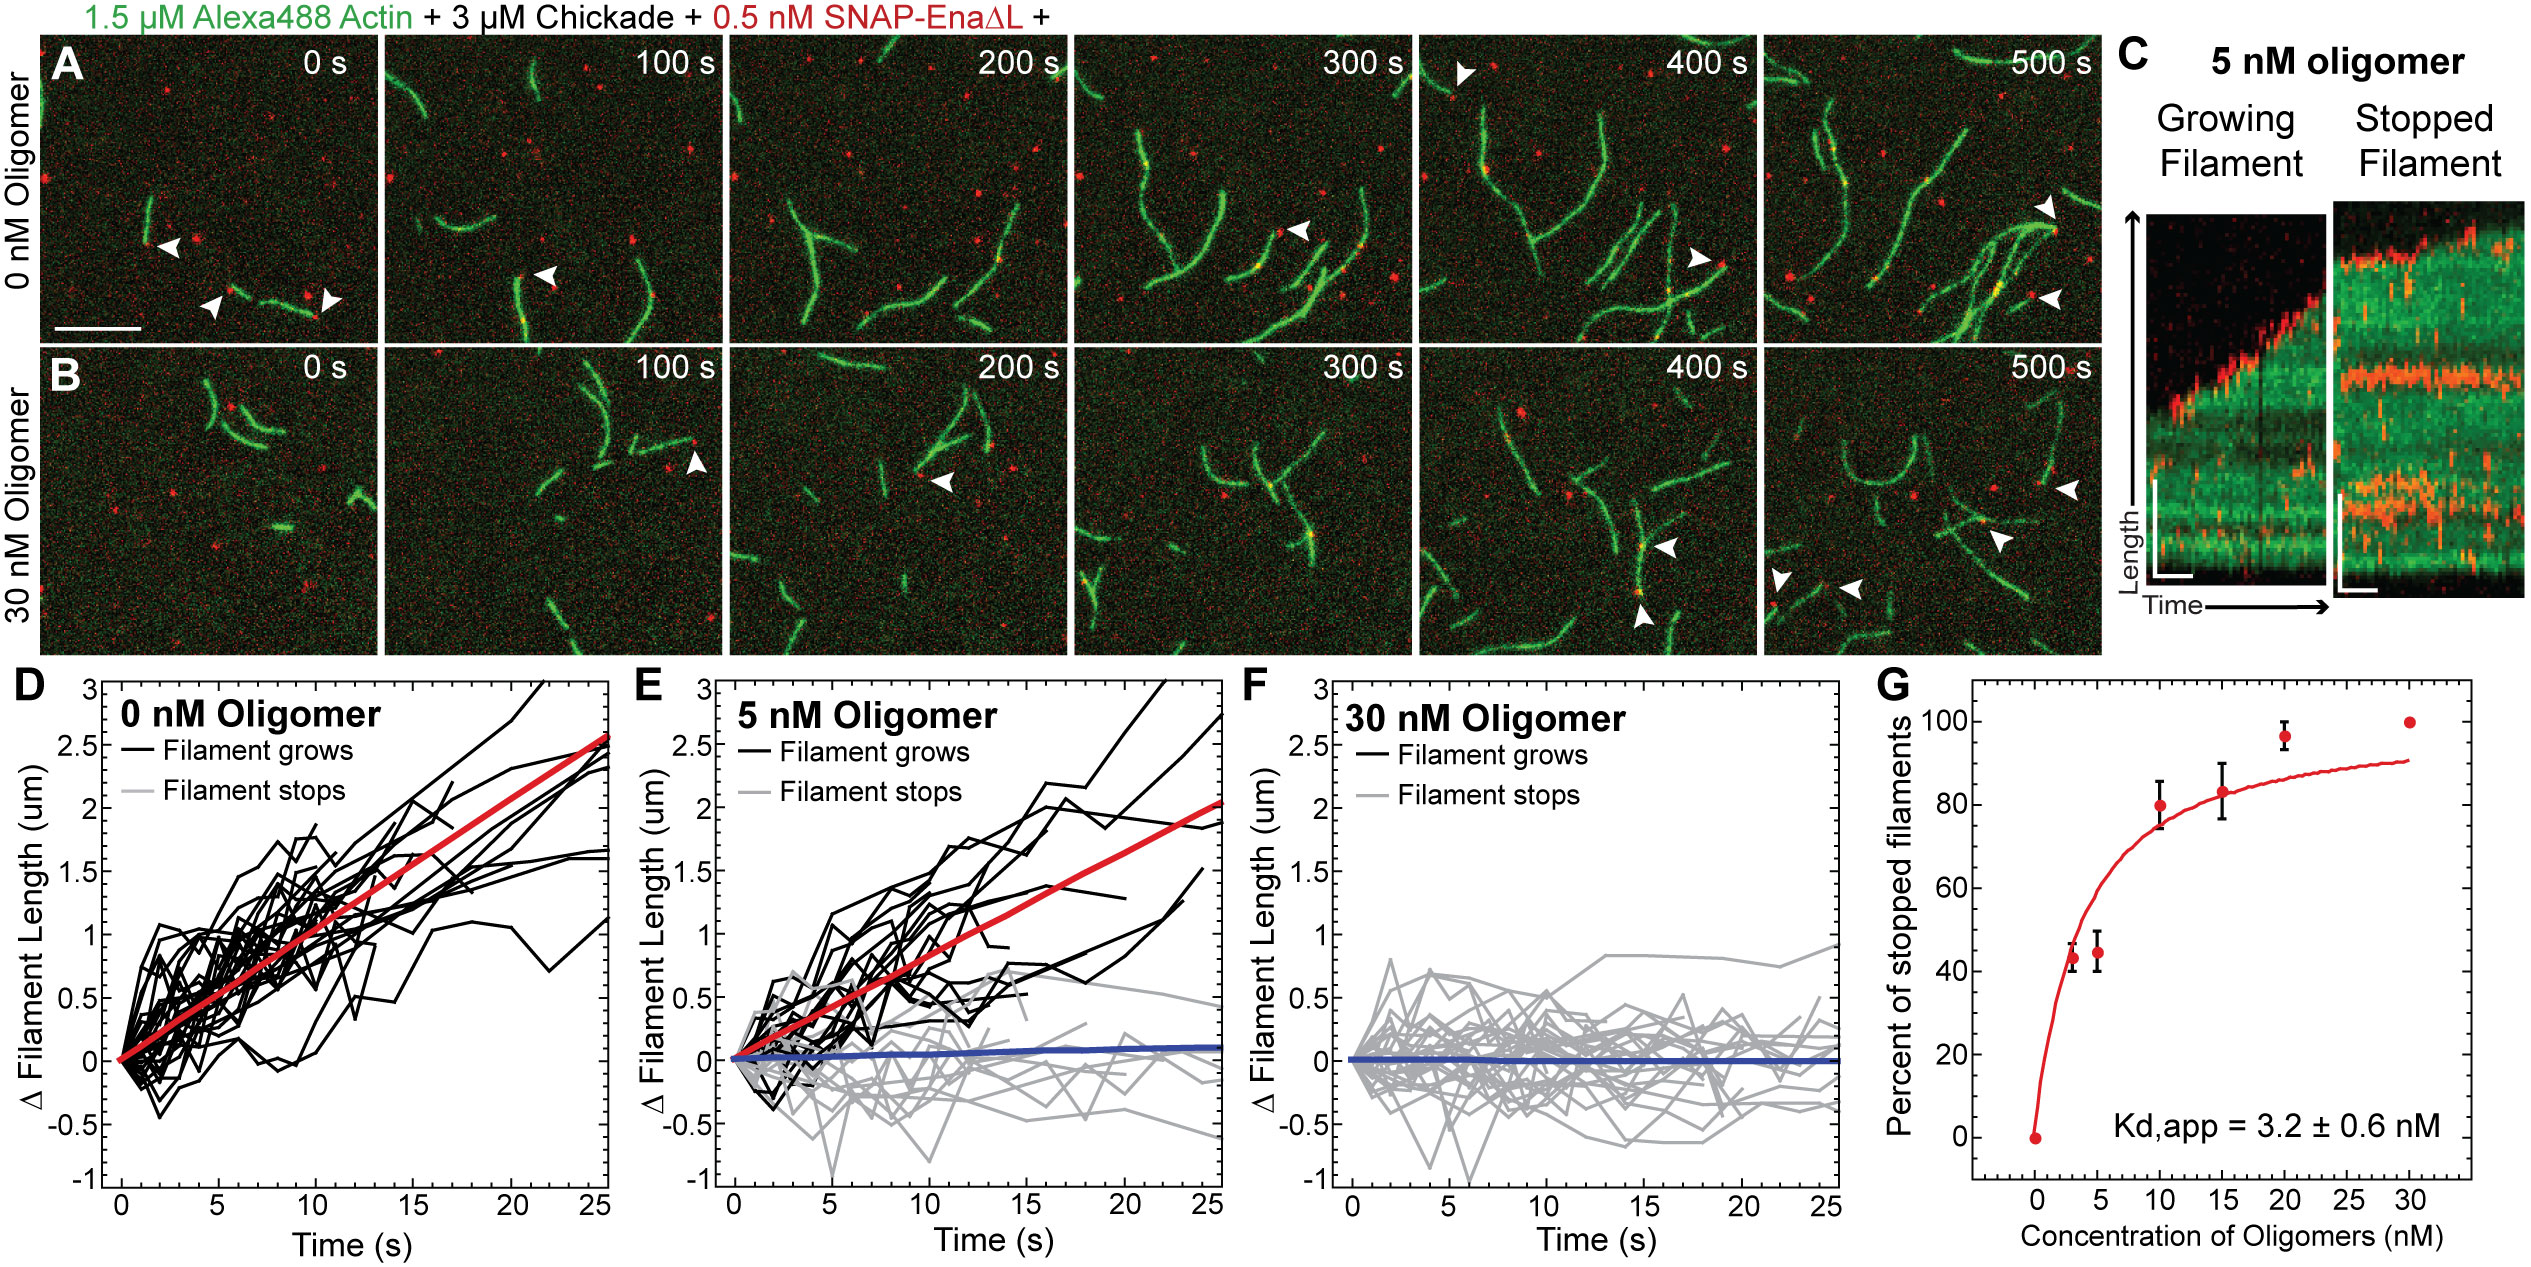
\includegraphics[width=\textwidth]{img/ch04/Oligomer_Ena_Figure.jpg}
\caption[Actin oligomers stop Ena mediated processive filament elongation.]{\textbf{Actin oligomers stop Ena mediated processive filament elongation.} Two color TIRFM timelapse of 1.5 $\mu$M Alexa-488 actin (green) and 0.5 nM SNAP-Ena$\Delta$L (red) in the presence of 3 $\mu$M Chickadee (fly profilin) and A) no actin oligomers or B) 30 nM actin oligomers. Arrows indicate Ena bound barbed ends. Scale bar, 10 $\mu$m. Kymographs of a G) growing Ena bound filament and a H) stopped Ena bound filament. Scale bar, 4 $\mu$m and 10 s. Filament elongation traces of Ena bound filaments with D) 0 nM Oligomers, E) 5 nM Oligomers, and F) 30 nM Oligomers. Red fit lines show average growth rates of Ena bound growing filaments and blue fit lines show average growth rates of Ena bound stopped filaments. C) Kd,app determined by TIRFM as percent of Ena bound stopped filaments over a range of actin oligomers. \textbf{Figure modified from \citep{kudryashova_actin_2018}}}
\label{fig:ena-oligomers}
\end{figure}

\subsection{VopL and VopF assemble endogenous actin}\label{vops}
To investigate the molecular mechanism of VopL/F actin nucleation we wanted to directly visualize labeled VopL/F using single-molecule TIRFM. We assembled 1.5 $\mu$M Mg-ATP-actin (15\% Oregon green-labeled) in the presence of 0.2 nM 549-SNAP-VopL/F to measure the elongation rate of actin filaments and the lifetime of VopL/F bound (Figure \ref{fig:vop}E-F). We observed that in the presence of growing filaments, VopL/F nucleate actin polymerization and bind to one end of actin filament as it continues to elongate. Barbed end associating proteins are known to typically affect the elongation rate of F-actin while they are bound (ie formins \citep{kovar_molecular_2006}). Therefore, we measured the elongation rate of VopL/F bound filaments (\mytilde13.0 sub/s) and found no difference in elongation rate compared to control filaments (Figure \ref{fig:vop}B-C). We measured the residence time of VopL and VopF to understand its dynamics on ends of filaments. Kaplan-Meier plots were used to calculate the average lifetime of bound VopL/F after nucleating the actin filament. To account for dead time required to flow in the reaction (\mytilde20 s) and for the resolution of the microscope to observe nascent filaments (\mytilde0.5 $\mu$m), we calculated two different residence times. The first residence time ($\tau$\textsubscript{Obs}) is from the observed timepoint where an actin filament and VopL/F protein are first visualized with TIRFM. The second residence time ($\tau$\textsubscript{Calc}) takes into account how long before the filament is able to be visualized due to the resolution of TIRFM. Overall we observe that both VopL and VopF bind to the end of filaments for a similar amount of times using either the observed residence time (VopL\textsubscript{Obs} $\tau$ = 35 s, VopF\textsubscript{Obs} $\tau$ = 27 s) or the calculated residence time (VopL\textsubscript{Calc} $\tau$ = 104 s, VopF\textsubscript{Calc} $\tau$ = 110 s). By creating kymographs of the filaments over time we see that the end that VopL/F binds to is the pointed, slow-growing end. Another way to visualize the pointed end in TIRFM is by using the fluorescence intensity along a filament. Due to photobleaching, the pointed end is dimmer than the newly assembled actin at the barbed end (Figure \ref{fig:vop}F). We see using linescans that VopL/F associate with this dimmer, pointed end (Figure \ref{fig:vop}H-I). In contrast, mDia2, a known barbed end-binding protein, binds to the brighter barbed end using linescans (Figure \ref{fig:vop}J). Therefore, VopL/F nucleates filaments and then binds to the dimmer, pointed end of F-actin for \mytilde110 s.

\begin{figure}
\centering
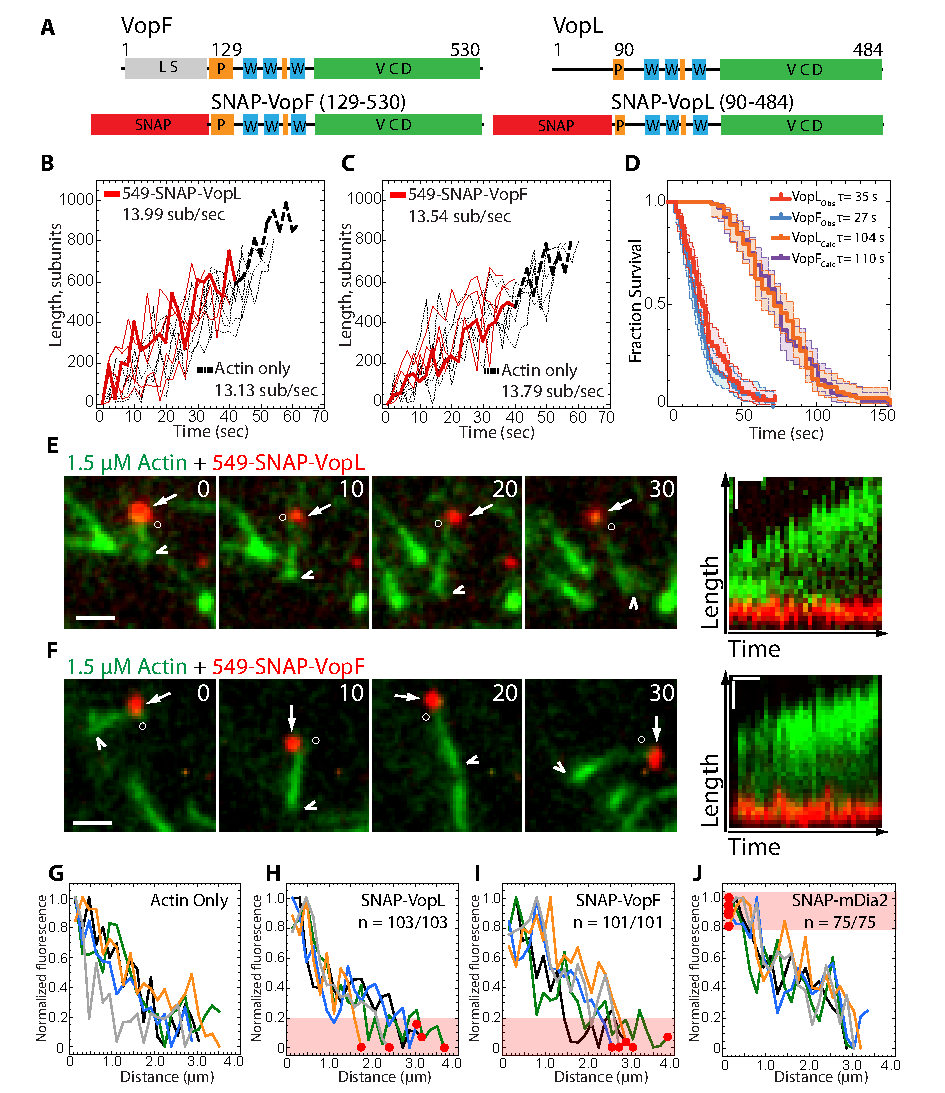
\includegraphics[width=\textwidth]{img/ch04/Thesis_Vop.pdf}
\caption[ VopL/F nucleate and then remain briefly associated with the pointed end of an actin filament.]{\textbf{ VopL/F nucleate and then remain briefly associated with the pointed end of an actin filament.} (A) Top, domain organization of VopL/F. Orange, proline-rich region (P); blue, WH2 domain (W); green, VCD dimerization domain. Bottom, VopL/F constructs used in this study with SNAP tag (red) for labeling. }
\label{fig:vop}
\end{figure}

% Continues caption on next page. Requires package ccaption.
\begin{figure}[!htb]
  \contcaption{(continued) (B–J) Slow acquisition (every 2 s, B–D) and rapid acquisition (every second, E–J) two-color TIRFM of the assembly of 1.5 $\mu$M Mg-ATP-actin (15\% Oregon green actin) with 0.2 nM 549(red)-SNAP-VopL/F. (B and C) Length of individual control (dashed black), 549-SNAP-VopL–associated (B, solid red), or 549-SNAP-VopF-associated (C, solid red) filaments over time ($n \geq 20$). (D) Kaplan–Meier curves representing the mean residence time of 549-SNAP-VopL/F on actin filaments observed (VopL\textsubscript{Obs}, VopF\textsubscript{Obs}) or assumed to have been associated because of nucleation (VopL\textsubscript{Calc}, VopF\textsubscript{Calc}). Error bars indicate 95\% CI; $n \geq 90$ events. (E and F, left) Merged timelapse micrographs (in seconds) of individual filaments. White arrowheads and open circles indicate bright and dim filament ends. White arrows indicate 549-SNAP-VopL/F. (E and F, right) Merged kymographs of filament length (y axis; bar, 1 $\mu$m) over time (x axis; bar, 10 s) of the corresponding filaments. Bars, 2 $\mu$m.  (G–J) Linescans of the normalized fluorescence intensity of individual actin filaments measured from their bright to dim (bleached) ends. Red dots indicate position of 549-SNAP-VopL/F or 549-SNAP-mDia2 on the filament traces, and shaded red regions indicate where 100\% of VopL/F or mDia2 are bound to the filaments (n $\geq$ 75). \textbf{TIRFM, elongationm and linescan analysis completed by Tom Burke. Figure modified from \citep{burke_bacterial_2017}.}}
\end{figure}

\section{Materials and Methods}\label{mat-meth-vib}
\subsection{ACD oligomer and Ena TIRFM}\label{oligo-mm-tirf}
TIRFM images were collected at 1s intervals with a cellTIRF 4Line system (Olympus, Center Valley, PA) fitted to an Olympus IX-71 microscope with through-the-objective TIRF illumination and an iXon EMCCD camera (Andor Technology, Belfast, UK). Mg-ATP-actin (15\% Alexa 488 labeled) was mixed with polymerization TIRF buffer [10 mM imidazole (pH 7.0), 50 mM KCl, 1 mM MgCl\textsubscript{2}, 1 mM EGTA, 50 mM DTT, 0.2 mM ATP, 50 $\mu$M CaCl\textsubscript{2}, 15 mM glucose, 20 $\mu$g/mL catalase, 100 $\mu$g/mL glucose oxidase, and 0.5\% (400 centipoise) methylcellulose] to induce F-actin assembly and 0.5 nM SNAP(549)-Ena$\Delta$L, 3 $\mu$M chickadee, and the noted concentration of ACD oligomers. This mixture was transferred to a flow cell for imaging at room temperature. For two color TIRFM, we cyclically imaged labeled actin (1 frame, 488 nm excitation for 50ms) and SNAP(549)-Ena$\Delta$L (1 frame, 561 nm excitation for 50ms) \citep{winkelman_ena/vasp_2014}. 

\subsection{Analysis of Ena/VASP elongation}
Barbed end elongation rates were calculated by measuring filament lengths over time with ImageJ software. Multiple filament lengths were plotted over time and the distribution was fit with a linear equation using KaleidaGraph 4.5 (Synergy Software, Reading, PA).

\subsection{Analysis of VopL/F lifetime}
Residence times for 549-SNAP-VopL/F on nucleated actin filaments in spontaneous TIRFM assays were determined through back-calculation by measuring the length of actin filaments immediately before the 549-SNAP-VopL/F dissociated and converting that length into total actin subunits (1 $\mu$m = 375 subunits). The subunit length was divided by the mean elongation rate of the filaments. Barbed-end elongation rates were calculated by measuring filament lengths over time with ImageJ. Residence times for single SNAP(549)-VopL/F dimers were determined by fitting a Kaplan-Meier \citep{kaplan_nonparametric_1958} survival curve with a single exponential equation, $f(x) = x_{0} * exp^{(-x/\tau)}$ to calculate the average lifetime. Kaplan Meier survival curves were used to account for processive runs that started before imaging began or ends after imaging terminated. Log rank statistical significance tests were done using Prism 7 (GraphPad Software, San Diego, CA). We reported two average lifetimes, one from observed time bound and other that is calculated accounting for the dead time required to flow the reaction into the chamber (\mytilde20 s) and for the filaments to reach an observable length (\mytilde0.5 $\mu$m).


